\documentclass[main.tex]{subfiles}
\begin{document}
% Explanation of the question
In this section, we are concerned with minimal injective resolutions of $\mathfrak{sp}_\infty-$ modules. In particular, we want to find the length and explicitly describe the last term of such resolutions.\\ 

% INTUITIVE ALGORITHM
We start by describing an algorithm for computing minimal injective resolutions of simple tensor $\mathfrak{sp}_\infty-$modules. Let us denote by $\Gamma_\lambda^k$ the $k$-th term in the injective resolution $$0\to\Gamma_{<\lambda>}\tof{\alpha_0}\Gamma_{\lambda} = \Gamma_\lambda^0\tof{\alpha_1} \Gamma_\lambda^1\tof{\alpha_2} ...\tof{\alpha_{s}}\Gamma_\lambda^s \to 0.$$

To calculate  $\Gamma_\lambda^k,$ we follow the steps below:
\begin{enumerate}
    \item $\Gamma_\lambda^1$ equals the injective hull $\bigoplus\limits_{\mu}\Gamma_\mu$ of all constituents $\Gamma_{<\mu>}$ of $\soc{2}\Gamma_\lambda$, and
    $$\im{\alpha_1}= 
    \begin{tabular}{|c|}
        \hline
        \vdots \\
        \hline $\soc{4}\Gamma_\lambda$ \\
       \hline $\soc{3}\Gamma_\lambda$ \\
        \hline $\soc{2}\Gamma_\lambda$ \\
        \hline
    \end{tabular}$$
    
    \item The next resolution term $\Gamma_\lambda^2$ equals the injective hull $\bigoplus\limits_\eta\Gamma_\eta$ of all simple constituents $\Gamma_{<\eta>}$(with possible repetitions) of $(\soc{2} \Gamma_\lambda^1)/\alpha_1(\soc{3}\Gamma_\lambda)$. The image of $\alpha_2$ is the composition of the surjection $\Gamma_\lambda^1\to\Gamma_\lambda^1/\;im\alpha_1$ with the injection of $\Gamma_\lambda^1/\;im\alpha_1$ into its injective hull. This injective hull coincides with the injective hull of $(\soc{2}\Gamma_\lambda^1)/(\soc{3}\Gamma_\lambda).$

    \item By repeating the method described above, one can compute all the next resolution terms $\Gamma_\lambda^{k+1}$ as the injective hull of all the modules of $(\soc{2} \Gamma_\lambda^k)/\alpha_k(\soc{3}\Gamma_\lambda^{k-1}).$  
\end{enumerate}

\bigskip

The fact that the so described algorithm is valid follows from the results of \cite{dancohen2012koszulcategoryrepresentationsfinitary} and \cite{SAM_2015}. \\

Given this algorithm, let us take an actual example, showcasing the steps.

\bigskip

\begin{ex}
\label{compute-res}
In this example, we show that the injective resolution of $\Gamma_{<(3,1,1,1)>}$ is 
$$0\to\Gamma_{<(3,1,1,1)>}\tof{\alpha_0}\Gamma_{(3,1,1,1)}\tof{\alpha_1}\Gamma_{(3,1)}\oplus\Gamma_{(2,1,1)}\tof{\alpha_2}\Gamma_{(2)} \oplus \Gamma_{(1,1)}\tof{\alpha_3}\Gamma_{\emptyset}\tof{\alpha_4} 0.$$

 We start by writing the 0-term of the injective resolution of $\Gamma_{<(3,1,1,1)>}:$  $$\Gamma_{(3,1,1,1)}^0 = \Gamma_{(3,1,1,1)}, $$ with socle filtration 
 $$
    \begin{tabular}{|c|}
        \hline $\Gamma_{<(2)>}$ \\
       \hline $\Gamma_{<(3,1)>}\oplus \Gamma_{<(2,1,1)>}$ \\
        \hline $\Gamma_{<(3,1,1,1)>}$ \\
        \hline
    \end{tabular}.
 $$
 
 In step 1, we find the injective hull of $\Gamma_{<(3,1)>}\oplus \Gamma_{<(2,1,1)>}$, and we obtain $\Gamma_{(3,1,1,1)}^1 = \Gamma_{(3,1)}\oplus \Gamma_{(2,1,1)}$ and
 $$\im{\alpha_1}= 
    \begin{tabular}{|c|}
       \hline $\Gamma_{<(2)>}$ \\
        \hline $\Gamma_{<(3,1)>}\oplus\Gamma_{<(2,1,1)>}$ \\
        \hline
    \end{tabular}.$$

Step 2 claims that, since
$$
\Gamma_{(3,1,1,1)}^1 = \Gamma_{(3,1)}\oplus \Gamma_{(2,1,1)} = 
    \begin{tabular}{|c|}
       \hline $\Gamma_{<(2)>}$ \\
        \hline $\Gamma_{<(3,1)>}$ \\
        \hline
    \end{tabular}
    \oplus
    \begin{tabular}{|c|}
       \hline $\Gamma_{<(2)>}\oplus\Gamma_{<(1,1)>}$ \\
        \hline $\Gamma_{<(2,1,1)>}$ \\
        \hline
    \end{tabular}
$$
we obtain $\Gamma_{(3,1,1,1)}^2 = \Gamma_{(2)}\oplus\Gamma_{(1,1)}$ and 
$$
\im{\alpha_2}= 
    \begin{tabular}{|c|}
       \hline $\Gamma_{<(2)>}\oplus\Gamma_{<(1,1)>}$ \\
        \hline 
    \end{tabular}.
$$


 Repeating the instructions from the algorithm
 % $$ 
 % \Gamma_{(3,1,1,1)}^2 = \Gamma_{(2)} \oplus \Gamma_{(1,1)} = 
 %    \begin{tabular}{|c|}
 %       \hline  \\
 %       \hline $\Gamma_{<(2)>}$ \\
 %        \hline
 %    \end{tabular}
 %    \oplus
 %    \begin{tabular}{|c|}
 %       \hline $\Gamma_{<\emptyset>}$ \\
 %        \hline $\Gamma_{<(1,1)>}$ \\
 %        \hline
 %    \end{tabular}.
 %    $$
we get that $\Gamma_{(3,1,1,1)}^3$ is the injective hull of all simple constituents of 
    % $(\soc{2}\Gamma_{(3,1,1,1)}^2\oplus\alpha_1(\soc{4}\Gamma_{(3,1,1,1)}))/\alpha_2(\soc{3}\Gamma_{(3,1,1,1)}^1).$ 
$\soc{2}\Gamma_{(3,1,1,1)}^2/\alpha_2(\soc{3}\Gamma_{(3,1,1,1)}^1).$ 
Hence, $\Gamma_{(3,1,1,1)}^{3}=\Gamma_{\emptyset}$, which is the last term in the minimal injective resolution.
\end{ex}

\bigskip



If we continue to compute the resolution terms for a general case, we can notice certain patterns in the partitions parametrizing the terms of $\Gamma_\lambda^k$. The key result is that the resolution terms contain only modules $\Gamma_\mu$ with partitions $\mu$ such that $\LR{\lambda}{\mu}{\delta}\neq 0$ for column-quasi-symmetric (CQS) partitions $\delta$. This is implied by \cite{SAM_2015} (page 45) In other words, we have the following: 

\bigskip
% THEOREM SAM SNOWDEN
\begin{thm}
\label{thm-res}
    For any partition $\lambda$ and the corresponding $\mathfrak{sp}_\infty-$module $\Gamma_\lambda$, the terms of a minimal injective resolution of $\Gamma_{<\lambda>}$ are 
    $$
    \Gamma_\lambda^{k} = \bigoplus\limits_{\mu} \left( \sum\limits_{|\delta|=2k ,  \delta \text{CQS}} \LR{\lambda}{\mu}{\delta} \right) \Gamma_{\mu},
    \hspace{0.7cm} \text{ for } k = 1, ..., \left[\frac{n}{2}\right], n = |\lambda|.$$
\end{thm}

\bigskip

\begin{ex}
    \label{ex-resolution-proof-nr}
    Let us compare the claim in theorem \ref{thm-res} with the result in the above example \ref{compute-res}.  \\

    The verification for the $0^{th}$ term is straightforward. \\ 
    
    Next, we look for CQS-subpartitions $\delta$ of $(3,1,1,1)$ of degree $2.$ There is only one such partition: $\delta_1=(1,1).$ We have $\Gamma_{(3,1,1,1)}^1 = \Gamma_{(3,1)}\oplus \Gamma_{(2,1,1)},$ and both Young diagrams of $(3,1)$ and $(2,1,1)$ lead to the Young diagram of $(3,1,1,1)$ through a strict $(1,1)-$expansion, hence the needed Littlewood-Richardson coefficients are positive. \\ 
    
    Similarly, for the second resolution term, the only $CQS-$subpartition of degree $4$ of $(3,1,1,1)$ is $\delta_2 = (2,1,1)$. We want to check if $\Gamma_{(3,1,1,1)}^2 = \Gamma_{(2)} \oplus \Gamma_{(1,1)}$. By the Littlewood-Richardson rule, we can obtain one tableau of shape $(3,1,1,1)/(2,1,1)$ and weight $(2)$ (Pieri rule on Young diagrams), and one tableau of shape $(3,1,1,1)/(2,1,1)$ and weight $(1,1)$.\\
    
    For the last term, $\Gamma_{(3,1,1,1)}^{3}=\Gamma_{\emptyset}$, we have that $\LR{(3,1,1,1)}{\emptyset}{(3,1,1,1)}=1$ since $(3,1,1,1)$ is a CQS-partition. Moreover, it is the maximal CQS-subpartition of $(3,1,1,1)$.
\end{ex}

\bigskip

In a fashion similar to the previous section, we now want to have an explicit formula for the length of the minimal injective resolution, as well as for the modules in the last term of the resolution. In section 2, we looked for the maximal subpartition of the form $(2\gamma)^T$; now we have to search for the unique maximal CQS-subpartition of $\lambda$ and for a formula for its degree. \\

In the proof below, we will refer to a $CQS$ partition with only one row and one column as a \textbf{corner column-quasi-symmetric (CCQS)} partition.

\bigskip
% PROPOSITION MAXIMAL CQS SUBPARTITION
\begin{prop}
    \label{prop-maximal-cqs}
    Any partition $\lambda$ contains a unique maximal column-quasi-symmetric subpartition $\delta_{max}.$\\
    Moreover, $|\delta_{max}|=2\sum\limits_{i=1}^{m} \text{min} (\lambda_i-i+1, (\lambda^T)_i-i),$ where $m$ is the number of boxes on the main diagonal of the Young diagram of $\lambda$.
\end{prop}

\begin{proof}
    Let us start by recalling  that the number of boxes on column $i$ of the Young diagram of any partition $\delta$ is equal to the number of boxes on the $i^{th}$ row of the Young diagram of $\delta^T,$ i.e. $(\delta^T)_i$.
    % Let $b_i$ be the $i^{th}$ box on the main diagonal. The number of boxes in the same row and to the right of $b_i$ is $\delta_i-i$, and the number of boxes in the same column and below $b_i$ is $(\delta^T)_i-i.$ 
    Then, by definition \ref{def-cqs}, $\delta$ is a $CQS-$partition if for any index $i$ of main diagonal boxes, $$(\delta^T)_i-i=\delta_i-i+1.$$

    Next, given a partition $\lambda = (\lambda_1, \lambda_2, ..., \lambda_r)$ with $m$ boxes on the main diagonal (hence, $\lambda_i\geq i $ for $1\leq i\leq m,$ and $\lambda_i < i $ for $m <i\leq r$), we will construct the maximal $CQS-$subpartition $\delta_{max}$ of $\lambda$. The construction algorithm will lead to the uniqueness of $\delta_{max}$. \\
    
    
    Denote by $b_i$ the $i^{th}$ box on the main diagonal with $1\leq i\leq m.$ For each $b_i$ we want to find a maximal $CCQS-$partition $\delta(i)$ whose Young diagram has $b_i$ as its top left box, its row boxes fit in the $i^{th}$ row of the Young diagram of $\lambda$ (to the right of the main diagonal), and its column boxes fit in the $i^{th}$ column of the Young diagram of $\lambda$ (below the main diagonal). This way, we find the maximal $CQS$ subpartition by describing its Young diagram as the union of the Young diagrams of corner column-quasi-symmetric partitions with top left boxes on the main diagonal $\delta(i)$ for $1\leq i\leq m$: 
    \begin{itemize}
        \item We start by considering the Young diagram of $\delta(1)$ (the ``outer corner" Young diagram), which has the maximal possible number of boxes from row $1$ and column $1.$
        \item Then, the first ``inner corner" Young diagram of the $CCQS-$partition $\delta(2)$ consists of boxes from row $2$ and column $2$ of the Young diagram of $\lambda$. 
        \item We continue in this manner until $\delta(m)$ is constructed.
    \end{itemize}
    
      The Young diagram of $\delta_{max}$, i.e. the union of the Young diagrams of $\delta(1), \delta(2),..., \delta(m)$, is maximal because each $\delta(i)$ is maximal and $m$ is the last main diagonal box. The partition $\delta_{max}$ is $CQS$ since the necessary condition $(\delta_{max}^T)_i-i=(\delta_{max})_i-i+1, $ for $1\leq i\leq m,$ follows directly from the $CCQS$ property of each $\delta(i):$ $\;\; (\delta(i)^T)_1 = \delta(i)_1+1, $ for $1\leq i\leq m.$\\

    Hence, it is enough to obtain an explicit formula for each $\delta(i)$ in terms of $\lambda$ to show the existence.\\
    
    From the Young diagram of $\delta(i)$, the $CCQS-$partition's row has $$\delta(i)_1 \leq \lambda_i-i+1 \text{ boxes (including the box $b_i$)},$$ and its column has $$(\delta(i)^T)_1 \leq (\lambda^T)_i-i+1 \text{ boxes (including the box $b_i$).}$$ The partition $\delta(i)$ is $CCQS$, hence it must satisfy $(\delta(i)^T)_1 = \delta(i)_1+1$. This leads to the inequalities:
    $$\delta(i)_1 \leq \lambda_i-i+1 \text{ and } \delta(i)_1 \leq (\lambda^T)_i-i \Rightarrow 
    \delta(i)_1 \leq min( \lambda_i-i+1, (\lambda^T)_i-i).$$
    Therefore, by choosing $\delta(i)_1 = min( \lambda_i-i+1, (\lambda^T)_i-i),$ we have found the unique maximal $CCQS-$partition $\delta(i)$ that fits in the $i^{th}$ row and column, to the right and, respectively, below the box $b_i$ on the main diagonal of the Young diagram of $\lambda$. Explicitly, the partition is 
    $$\delta(i)= (\delta(i)_1, \underbrace{1, 1, ..., 1}_\text{$\delta(i)_1$ times}), \;\;\;\text{ with degree } |\delta(i)|= 2\delta(i)_1.$$

   The above implies that $\delta_{max},$ exists and is unique, and its degree is 
    $$
    |\delta_{max}| = \sum\limits_{i=1}^{m}|\delta(i)| = 2\sum\limits_{i=1}^{m}|\delta(i)_1|=2\sum\limits_{i=1}^{m} min(\lambda_i-i+1, (\lambda^T)_i-i).
    $$

\end{proof}

\bigskip

\begin{ex}
\label{ex-maximal-cqs}
    In this example, we find the maximal $CQS-$subpartition of $\lambda=(6,5,4,4,2,1,1)$. We start by drawing its Young diagram, as seen in figure \ref{fig:cqs-lambda}, and computing the conjugate partition $\lambda^T=(7,5,4,4,2,1)$. There are four boxes on the main diagonal of the Young diagrams of both $\lambda$ and $\lambda^T$, therefore we need to find four partitions $\delta(i),$ $1\leq i\leq 4.$ We compute each $\delta(i)_1$ and obtain the $CCQS-$partitions:
    $$
    \delta(1)_1 = min(\lambda_1, (\lambda^T)_1-1) = min(6,6) = 6 \; \; \Rightarrow \; \; \delta(1) = (6,1,1,1,1,1,1), 
    $$
    $$
    \delta(2)_1 = min(\lambda_2-1, (\lambda^T)_2-2) = min(4,3) = 3 \; \;\Rightarrow \; \; \delta(2) = (3,1,1,1),
    $$
    $$
    \delta(3)_1 = min(\lambda_3-2, (\lambda^T)_3-3) = min(2,1) = 1 \; \;\Rightarrow \; \; \delta(3)=(1,1),
    $$
    $$
    \delta(4)_1 = min(\lambda_4-3, (\lambda^T)_4-4) = min(1,0) = 0 \; \;\Rightarrow \; \; \delta(4) \text{is the empty partition}.
    $$
    
    Their Young diagrams can be seen in figure \ref{fig:cqs-delta-i}.\\
    
    \begin{figure}[H]
        \centering
        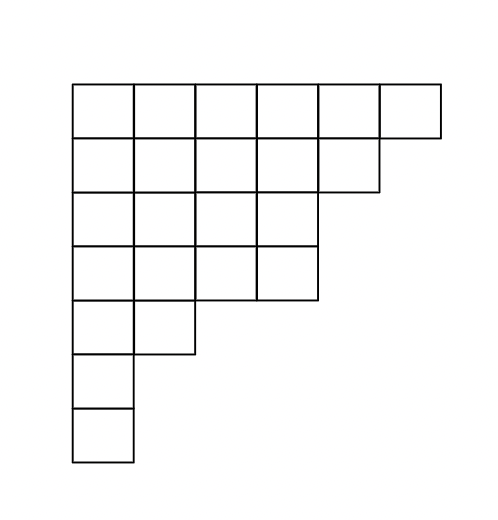
\includegraphics[width=0.25\linewidth]{images/CQS-lambda.png}
        \caption{Young diagram of $\lambda=(6,5,4,4,2,1,1)$}
        \label{fig:cqs-lambda}
    \end{figure}
    \begin{figure}[H]
        \centering
        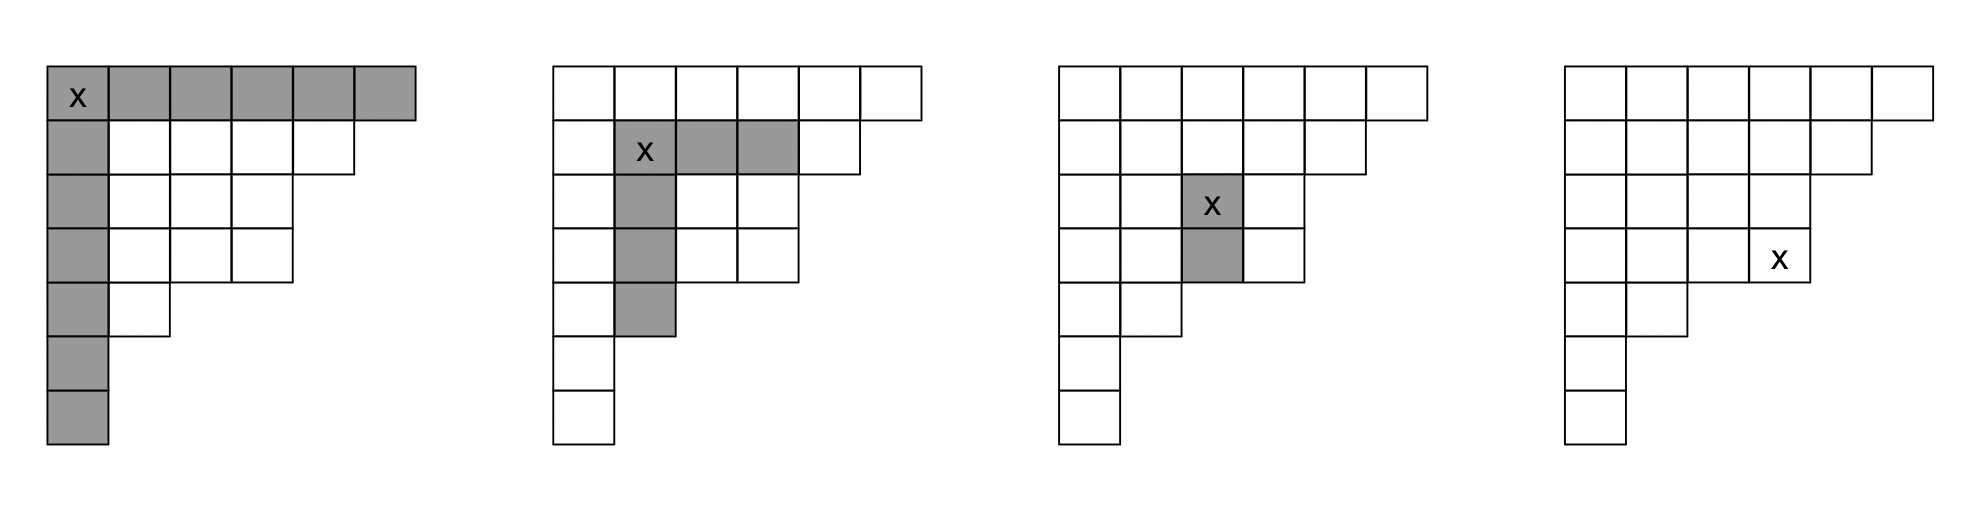
\includegraphics[width=0.9\linewidth]{images/CQS-delta-i.png}
        \caption{Highlighted, from left to right: $\delta(1), \delta(2), \delta(3), \delta(4)$ drawn on top of the Young diagram of $\lambda,$ for emphasis on their maximality. Boxes on the main diagonal are marked with an $\times$. }
        \label{fig:cqs-delta-i}
    \end{figure}

    The maximal $CQS-$subpartition $\delta_{max}$ is $(6,4,3,3,2,1,1)$, its Young diagram is graphical union of the Young diagrams of $\delta(1), \delta(2), \delta(3), \delta(4)$, and its degree is $20.$

    \begin{figure}[H]
        \centering
        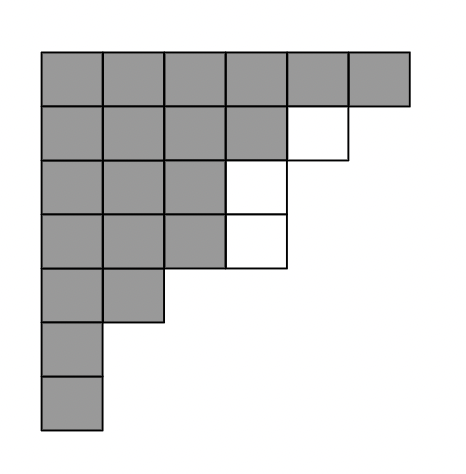
\includegraphics[width=0.25\linewidth]{images/CQS-delta-max.png}
        \caption{The Young diagram of the maximal CQS subpartition, inside the Young diagram of $\lambda.$ }
        \label{fig:cqs-delta-max}
    \end{figure}
\end{ex}

\bigskip
% PROPOSITION LAST TERM
\begin{prop}
\label{prop-last-res-term}
    For any partition $\lambda$, let $\delta_{\text{max}}$ be its maximal CQS-subpartition. Denote by $l$ the number of boxes in the longest column of the skew diagram $\lambda/\delta_{\text{max}}$. 
    Then the last nonzero term of a minimal injective resolution of the $\mathfrak{sp}_\infty-$module $\Gamma_{<\lambda>}$ has the form $\Gamma_\mu\oplus(\bigoplus\limits_{\eta}\Gamma_\eta)$ for some partition $\mu$ of length $l$ and possibly further partitions $\eta$ of length at least $l$ such that $|\mu| = |\eta|=|\lambda|-|\delta_{max}|,$ and not necessarily distinct to $\mu$.
\end{prop}

\begin{proof}
    We define the partition $\mu$ as $(c_1, c_2, c_3, ..., c_l),$ where $c_i$ is the number of columns of the skew diagram $\lambda/\delta_{\text{max}}$  with at least $i$ boxes, for all $i=1,...,l.$ To show that $\LR{\lambda}{\delta_{\text{max}}}{\mu}\geq 1$, we construct a Littlewood-Richardson tableau of shape $\lambda/\delta_{\text{max}}$ and weight $\mu.$ For this, we fill the boxes of the skew diagram $\lambda/\delta_{\text{max}}$ column by column, by placing $1$ in the top box of each column, then $2$ in the box below, $3$ in the next one, and so on, until the $l-$th box in the longest columns. This yields a Littlewood-Richardson tableau of $\lambda/\delta_{\text{max}}$ and weight $\mu,$ and by attaching the Young diagram of $\delta_{max}$ to this skew tableau, we realize $\lambda$ as a strict $\mu-$expansion of the Young diagram of $\delta_{max}$.  Hence, $\LR{\lambda}{\delta_{\text{max}}}{\mu}\geq 1$ by Theorem \ref{LR-comb-rule-tableaux}.\\
    
    Any other module $\Gamma_\eta$ appearing in the last nonzero term of the resolution must satisfy $\LR{\lambda}{\delta_{\text{max}}}{\eta}\geq 1,$ therefore there must exist at least one Littlewood-Richardson tableau of shape $\lambda/\delta_{\text{max}}$ and weight $\eta$. Since the skew diagram $\lambda/\delta_{\text{max}}$ contains at least a column of length $l,$ when filling its boxes to obtain a Littlewood-Richardson tableau of weight $\eta$, we are not allowed to place the same number twice in the same column. Hence the maximal columns need to contain $l$ distinct numbers, i.e. $\eta$ has length at least $l$. Therefore, there is no $\mathfrak{sp}_\infty-$module $\Gamma_\eta$ with length less than $l$ in the last term of the injective resolution of $\Gamma_\lambda$.\\
\end{proof}
\bigskip

\begin{ex}
    \label{ex-last-term-res}
    Let $\lambda = (4,3,3,2,2,2,2)$ be a partition with unique maximal $CQS$-subpartition $\delta_{max}=(4,3,2,2,1).$ We draw the Young diagram of $\delta_{max}$ inside the Young diagram of $\lambda$ (figure \ref{fig:max-cqs} ) and see that the semistandard skew tableau of shape $\lambda/\delta_{max}$ contains a column of length $1$, one of length $2$, and one of length $3$.\\
    \begin{figure}[H]
        \centering
        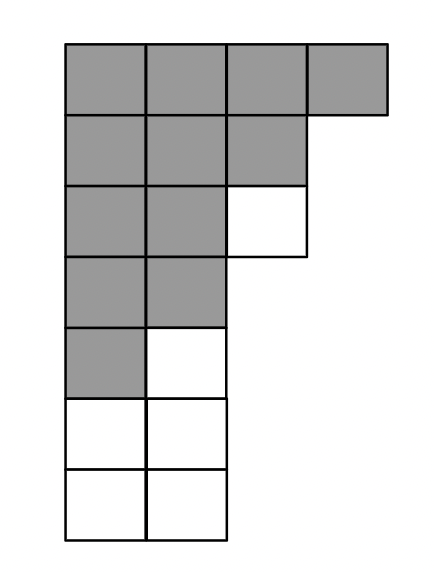
\includegraphics[width=0.2\linewidth]{images/MaxCQS.png}
        \caption{The Young diagram of the partition $(4,3,3,2,2,2,2),$ with the Young diagram of its maximal $CQS$-subpartition $(4,3,2,2,1)$ highlighted inside.}
        \label{fig:max-cqs}
    \end{figure}
    
    When numbering the boxes of the tableau according to the parts of a weight $\mu$, we must have a strictly increasing order on each column, so the length of $\mu$ is at least $3$. We see in figure \ref{fig:algorithm-res-last-term} that the partition $\mu=(3,2,1)$ defined as in the proof of Proposition \ref{prop-last-res-term} can serve as a weight for a Littlewood-Richardson tableau of shape $(4,3,3,2,2,2,2)/(4,3,2,2,1)$. Additionally, there exist other partitions $\mu$ of length at least 3 such that $\LR{\lambda}{\delta_{max}}{\mu}\neq 0$. Two of them are $(2,2,2)$ and $(2,2,1,1)$. These all satisfy the claim that the last nonzero term of a minimal injective resolution of $\Gamma_{<(4,3,3,2,2,2,2))>}$ has the form $\Gamma_{(3,2,1)}\oplus(\bigoplus\limits_{\eta}\Gamma_\eta),$ with $(3,2,1)$ of length $3$, and where the partitions $\eta$ are of length at least $3$ and $|\eta| = |(3,2,1)|= 6$.
    \begin{figure}[H]
        \centering
        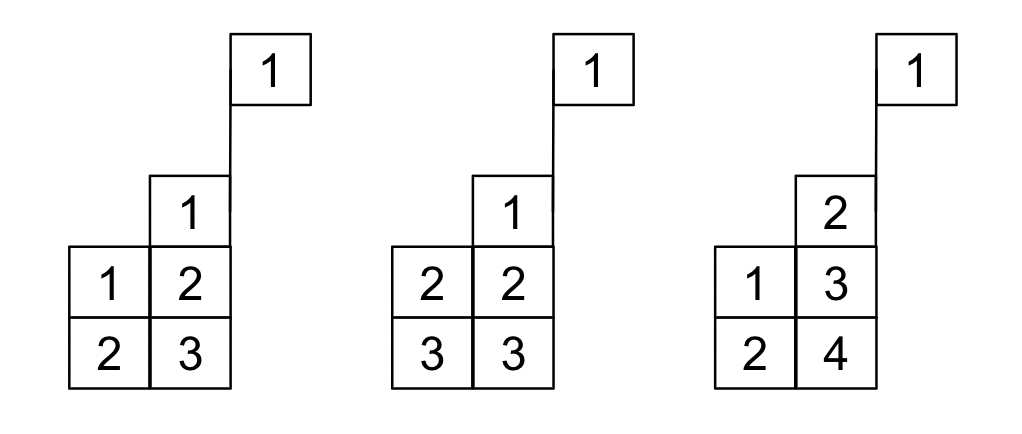
\includegraphics[width=0.5\linewidth]{images/TableauxAlgRes.png}
        \caption{Littlewood-Richardson tableaux of shape $(4,3,3,2,2,2,2)/(4,3,2,2,1)$ and weight $(3,2,1)$ (left), $(2,2,2)$ (middle), and $(2,2,1,1)$ (right). }
        \label{fig:algorithm-res-last-term}
    \end{figure}
\end{ex}

\begin{crl}
    \label{res-length}
    For any partition $\lambda$, let $\delta_{max}$ be its maximal column-quasi-symmetric subpartition. Then the length of a minimal injective resolution of the corresponding $\mathfrak{sp}_\infty-$module $\Gamma_{<\lambda>}$ is equal to $\frac{|\delta_{max}|}{2}+1.$
\end{crl}
\bigskip

\begin{crl}
    The $\mathfrak{sp}_\infty-$module $\Gamma_{\emptyset}$ appears as the last term of the injective resolution of some $\mathfrak{sp}_\infty-$module $\Gamma_{<\lambda>}$ if and only if the partition $\lambda$ is column-quasi-symmetric. 
\end{crl}

\bigskip
\end{document}